%! Author = Omar Iskandarani
%! Date = 12/3/2025
%! Affiliation = Independent Researcher, Groningen, The Netherlands
%! License = © 2025 Omar Iskandarani. All rights reserved. This manuscript is made available for academic reading and citation only. No republication, redistribution, or derivative works are permitted without explicit written permission from the author. Contact: info@omariskandarani.com
%! ORCID = 0009-0006-1686-3961
%! DOI = 10.5281/zenodo.17813283

\newcommand{\paperdoi}{10.5281/zenodo.17813283}
\newcommand{\papertitle}{{Multi--Scale Thermodynamics of the Swirl Condensate}\\[4pt]
{\large A Unified Hydrodynamic--Topological Framework for Swirl--String Theory}}

%=========================================
% PREAMBLE, PACKAGES AND DOCUMENT CONFIGURATION
%=========================================
\documentclass[11pt]{article}
\usepackage{amsmath,amssymb,amsfonts,bm}
\usepackage{siunitx}
\usepackage[hidelinks]{hyperref}
\usepackage[a4paper,margin=1in]{geometry}
\usepackage[T1]{fontenc}
\usepackage[utf8]{inputenc}
\usepackage{tikz}

%=========================================
% SST MACROS (GLOBAL)
%=========================================

% swirl arrows (context-aware)
\newcommand{\swirlarrow}{\mkern-2mu\scriptscriptstyle\boldsymbol{\circlearrowleft}}
\newcommand{\swirlarrowcw}{\mkern-2mu\scriptscriptstyle\boldsymbol{\circlearrowright}}

\newcommand{\vswirl}{\mathbf{v}_{\swirlarrow}}
\newcommand{\vswirlcw}{\mathbf{v}_{\swirlarrowcw}}
\newcommand{\SwirlClock}{S_{(t)}^{\swirlarrow}}
\newcommand{\SwirlClockcw}{S_{(t)}^{\swirlarrowcw}}

\newcommand{\Fmaxswirl}{F^{\max}_{\mkern-1mu\scriptscriptstyle\boldsymbol{\circlearrowleft}}}
\newcommand{\Fmaxswirlcw}{F^{\max}_{\mkern-1mu\scriptscriptstyle\boldsymbol{\circlearrowright}}}
\newcommand{\Fmax}{\Fmaxswirl}               % default maximal force (left swirl)
\newcommand{\FmaxEM}{F^{\max}_{\mathrm{EM}}}
\newcommand{\FmaxG}{F_{\mathrm{G}}^{\max}}   % G-like maximal force scale

\newcommand{\omegas}{\boldsymbol{\omega}_{\swirlarrow}}  % swirl vorticity
\newcommand{\Om}{\Omega_{\swirlarrow}}                   % swirl angular frequency profile

\newcommand{\vscore}{v_{\swirlarrow}}                    % shorthand: |v_swirl| at r=r_c
\newcommand{\vnorm}{\lVert \mathbf{v}_{\swirlarrow} \rVert} % swirl speed magnitude
\newcommand{\Ce}{\vswirl}                                % canonical swirl-speed constant

\newcommand{\rhof}{\rho_{\!f}}                           % effective fluid density
\newcommand{\rhoE}{\rho_{\!E}}                           % swirl energy density
\newcommand{\rhom}{\rho_{\!m}}                           % mass-equivalent density
\newcommand{\rhoM}{\rho_{\!m}}                           % alias
\newcommand{\rhocore}{\rho_{\text{core}}}                % core density
\newcommand{\rc}{r_c}                                    % string core radius (swirl string radius)

\newcommand{\Lam}{\Lambda}                               % Swirl Coulomb constant
\newcommand{\alpg}{\alpha_g}                             % gravitational fine-structure analogue

%=========================================
% Title page helpers
%=========================================
\newcommand{\titlepageOpen}{
    \begin{titlepage}
    \thispagestyle{empty}
    \centering
    \Large \bfseries \papertitle \par \vspace{1cm}
    {\Large \itshape \textbf{Omar Iskandarani}\textsuperscript{\textbf{*}} \par}
    \vspace{0.5cm}
    {\today \par}
    \vspace{0.5cm}
}

\newcommand{\titlepageClose}{
    \vfill \raggedright \null
    \begin{picture}(0,0)
    \put(0,-45){
        \begin{minipage}[b]{0.7\textwidth} \footnotesize
        \renewcommand{\arraystretch}{1.0}
        \noindent\rule{\textwidth}{0.4pt} \\[0.5em]
        \textsuperscript{\textbf{*}} Independent Researcher, Groningen, The Netherlands \\
        Email: \texttt{info@omariskandarani.com} \\
        ORCID: \texttt{\href{https://orcid.org/0009-0006-1686-3961}{0009-0006-1686-3961}} \\
        DOI: \href{https://doi.org/\paperdoi}{\paperdoi}
        \end{minipage}
    }
    \end{picture}
    \end{titlepage}
}

%=========================================
% Start Document - Title Page
%=========================================
\begin{document}
    \titlepageOpen
    \begin{abstract}
        We develop a comprehensive thermodynamic formulation of Swirl--String Theory (SST),
        in which the physical vacuum is modeled as a frictionless, incompressible swirl
        condensate, and all matter arises as topologically stabilized vortex filaments
        (``swirl strings''). Building on the quantum--thermodynamic isomorphism of Abe \&
        Okuyama, we demonstrate that hydrogenic structure, particle masses, vacuum
        fluctuations, and interaction lifetimes can be reinterpreted as thermodynamic
        processes involving the swelling, compression, and mode--excitation of vortex
        cores.

        We define SST Work as the mechanical energy required to deform the vortex core
        radius against the surrounding swirl pressure, and SST Heat as the energy
        redistributed among Kelvin modes and topological phase channels. Applying this
        framework to hydrogen, we show that the Bohr radius is not a probabilistic orbital
        shell but a thermodynamic equilibrium surface where centrifugal swirl pressure
        balances vacuum tension.

        We reinterpret the Golden Layer mass hierarchy as a discrete thermodynamic
        scaling law governed by the golden ratio, emerging from log--periodic structure in
        the swirl energy density. The Unruh Echo is shown to arise from a two--stage
        thermodynamic response: a 0.1 ns vorticity burst followed by a delayed
        electromagnetic transduction pulse around 30 ns. Finally, we derive partition
        functions, heat capacities, and provide numerical evaluation for a simplified
        Golden ladder.
    \end{abstract}

    \titlepageClose

%==============================================================
%  MULTI-SCALE THERMODYNAMICS OF THE SWIRL CONDENSATE — DEEL I
%==============================================================

%==============================================================
    \section{Introduction: The Hydrodynamic Necessity}
%==============================================================

        \subsection{Ontological Divergence in Modern Physics}

            General Relativity models gravity as spacetime curvature, while Quantum Field
            Theory models matter as excitations of an operator--valued vacuum. These
            frameworks are empirically successful yet mathematically incompatible.

            Swirl--String Theory (SST) replaces both ontologies with a physical one: the
            vacuum is a real fluid with density, pressure, vorticity, and circulation. Matter
            is reinterpreted as knotted vortex filaments of this medium. Mass, time dilation,
            charge, binding energy and field structure all emerge as hydrodynamic responses.

        \subsection{The Thermodynamic Hypothesis}

            SST has precise formulations for kinematics, field analogues, knot mass spectra,
            and hydrogen structure, but lacks a unifying thermodynamic interpretation.
            Abe \& Okuyama showed that the Schrödinger equation can be reformulated as a
            thermodynamic equation of state if one assigns Shannon entropy to the quantum
            probabilities and imposes the Clausius equality.\footnote{S.~Abe and S.~Okuyama,
        ``Similarity between quantum mechanics and thermodynamics: Entropy, temperature,
        and Carnot cycle,'' Phys.\ Rev.\ E \textbf{83}, 021121 (2011).}
            Their mapping between probability flows and thermodynamic heat is the missing
            bridge for SST.

        \subsection{Objectives of this Framework}

            Our aims:
            \begin{enumerate}
                \item Define the swirl string as a thermodynamic system embedded in a reservoir.
                \item Identify its thermodynamic variables: core radius, Kelvin modes, topology.
                \item Define SST Work as geometric deformation of $\rc$.
                \item Define SST Heat as Kelvin--mode or R/T--phase redistribution.
                \item Derive the SST equation of state from Euler--Bernoulli and circulation laws.
                \item Map Abe--Okuyama adiabatic/isothermal processes to SST swelling dynamics.
                \item Apply the framework to hydrogen, Golden Layers, Unruh Echo and partition
                functions.
            \end{enumerate}

%==============================================================
    \section{The Hydrodynamic Substrate: Axioms and Constants}
%==============================================================

        \subsection{The Primitive Triad}

            SST is based on three primitive medium parameters:
            \begin{itemize}
                \item Circulation quantum:
                \begin{equation}
                    \Gamma_0 \approx 6.4 \times 10^3 \ \mathrm{m^2/s}.
                \end{equation}

                \item Core radius:
                \begin{equation}
                    \rc \approx 1.41 \times 10^{-15} \ \mathrm{m}.
                \end{equation}

                \item Effective fluid density:
                \begin{equation}
                    \rhof \approx 7.0 \times 10^{-7} \ \mathrm{kg/m^3}.
                \end{equation}
            \end{itemize}

            Via circulation conservation $\Gamma = v r$, this yields the swirl speed scale
            \begin{equation}
                v_{\!\circlearrowleft} = \frac{\Gamma_0}{2\pi \rc}
                \approx 1.09 \times 10^6 \ \mathrm{m/s}.
            \end{equation}
            This is the characteristic ``sound'' speed of swirl excitations.

        \subsection{The Mass Kernel as Equation of State}

            SST mass arises from the hydrodynamic energy of the vortex:
            \begin{equation}
                M(T) = \Lambda_0 \, \mathcal{I}_M(K(T)) \, L_{\rm tot}(T),
            \end{equation}
            with $\Lambda_0 \propto \rhof v_{\!\circlearrowleft}^2 \rc^3$, a topological
            invariant $\mathcal{I}_M$, and total ropelength $L_{\rm tot}$.
            Thus rest mass is interpreted as stored adiabatic work.

        \subsection{The Swirl Clock}

            Time dilation follows:
            \begin{equation}
                S_t = \sqrt{1 - \frac{v^2}{c^2}}.
            \end{equation}
            Since $v \sim 1/r$, smaller radii produce larger speeds and slower clocks.
            This couples energy density directly to local temporal flow.

%==============================================================
    \section{The Quantum--Thermodynamic Isomorphism (Abe--Okuyama)}
%==============================================================

        \subsection{Particle in a Box vs.\ Vortex in a Core}

            Quantum energies scale as:
            \begin{equation}
                E_n(L) \propto \frac{1}{L^2}.
            \end{equation}
            Vortex energies scale as:
            \begin{equation}
                E(\rc) \propto \frac{1}{\rc^2}.
            \end{equation}
            Hence the mappings:
            \begin{equation}
                L \leftrightarrow \rc, \qquad
                |u_n\rangle \leftrightarrow \text{Kelvin modes}.
            \end{equation}

        \subsection{Mapping of Variables}

            \begin{center}
                \begin{tabular}{lll}
                    \hline
                    Abe--Okuyama          & SST Equivalent        & Interpretation \\
                    \hline
                    Well width $L$        & Core radius $\rc$     & Confinement scale \\
                    Probabilities $p_n$   & Kelvin mode weights   & Microstates \\
                    Heat                  & $\sum E_n dp_n$       & Mode excitation \\
                    Work                  & $\sum p_n dE_n$       & Core deformation \\
                    Entropy               & Shannon entropy       & Topological/Modal complexity \\
                    \hline
                \end{tabular}
            \end{center}

        \subsection{First and Second Laws}

            Quantum variation:
            \begin{equation}
                dE = \sum_n E_n dp_n + \sum_n p_n dE_n.
            \end{equation}
            Thus:
            \begin{equation}
                \delta Q = \sum_n E_n dp_n, \qquad
                \delta W = \sum_n p_n dE_n.
            \end{equation}

            In SST:
            \begin{itemize}
                \item Heat = redistribution of Kelvin modes.
                \item Work = deformation of $\rc$.
            \end{itemize}

        \subsection{Summary comparison: Abe--Okuyama vs.\ SST}
            The Abe--Okuyama (AO) framework treats thermodynamics as an
            information--theoretic structure defined on a fixed Hilbert space.
            Temperature appears as a Lagrange multiplier enforcing a constraint
            on the Shannon entropy of expansion probabilities, and no physical
            medium is introduced. In Swirl--String Theory (SST), by contrast,
            thermodynamics is mechanical: temperature, heat, and work are
            properties of a continuous swirl condensate and its topological
            defects.

            In AO, the microscopic degrees of freedom are the amplitudes
            $\{c_n\}$ or probabilities $\{p_n\}$ in an energy eigenbasis
            $\{|u_n\rangle\}$; the geometry of space does not deform when the
            system is heated or cooled. Heat is associated with changes
            ${\rm d}p_n$ at fixed spectrum $\{E_n\}$, while work is associated
            with changes in the spectrum ${\rm d}E_n$ at fixed $\{p_n\}$ due to
            external parameter variation (e.g.\ moving the walls of a box of
            width $L$).

            In SST, the microscopic degree of freedom is the radius of a
            swirl core and its surrounding equilibrium boundary. The relevant
            strain variable is the geometric deformation
            of the core/orbital radius away from equilibrium, encoded in the
            swirl temperature $T_{\text{swirl}}$. Heat corresponds to the
            excitation and damping of Kelvin modes and topological channels
            at fixed core radius, while work is the mechanical swelling or
            compression of the core against the ambient swirl pressure.

            These different ontologies lead to distinct equations of state for
            the energy--temperature relationship. SST predicts a quadratic
            low--temperature law for the swelling mode,
            \begin{equation}
                E_{\text{SST}}(T_{\text{swirl}})\;\propto\;T_{\text{swirl}}^{2},
                \qquad
                C_V^{\text{SST}}(T_{\text{swirl}})\;\equiv\;
                \frac{{\rm d}E_{\text{SST}}}{{\rm d}T_{\text{swirl}}}
                \;\propto\;T_{\text{swirl}},
            \end{equation}
            whereas a gapped AO two--level truncation yields a Schottky--type
            behavior
            \begin{equation}
                C_V^{\text{AO}}(T)\;\propto\;\left(\frac{\Delta E}{k_B T}\right)^2
                \exp\!\left(-\frac{\Delta E}{k_B T}\right),
            \end{equation}
            vanishing exponentially as $T\to 0$ and approaching a constant
            high--temperature limit. The qualitative contrast
            $C_V^{\text{SST}}\sim T_{\text{swirl}}$ vs.\
            $C_V^{\text{AO}}\sim\exp(-\Delta E/k_B T)$ provides a clear
            empirical discriminator between the two vacua, and will be used
            below as the basis for low--temperature and log--periodic heat
            capacity tests.

            \begin{table}[t]
                \centering
                \small
                \begin{tabular}{p{3cm}p{5.4cm}p{5.4cm}}
                    \hline
                    Feature & Abe--Okuyama (AO) & Swirl--String Theory (SST) \\
                    \hline
                    Ontology
                    & Pure states in Hilbert space; no explicit medium
                    & Physical swirl condensate with density, pressure, vorticity; particles are knotted defects \\
                    Temperature
                    & Lagrange multiplier enforcing the Clausius relation for Shannon entropy
                    & Geometric strain of an equilibrium boundary; $T_{\text{swirl}} = \Theta\,\epsilon$ encodes radial swelling \\
                    Heat $Q$
                    & Energy change from ${\rm d}p_n$ at fixed spectrum $\{E_n\}$
                    & Kelvin--mode and topological excitation at fixed core radius $\rc$ \\
                    Work $W$
                    & Energy change from ${\rm d}E_n$ at fixed $\{p_n\}$ via external parameter variation (e.g.\ box width $L$)
                    & Mechanical swelling/compression of the core and orbital envelope against vacuum swirl pressure \\
                    Equation of state
                    & Low--$T$ energy changes governed by gapped spectrum; two--level truncation gives Schottky behavior
                    & Swelling mode obeys $E_{\text{SST}} \propto T_{\text{swirl}}^{2}$ for small strain, defining an elastic equation of state \\
                    Heat capacity $C_V$
                    & $C_V^{\text{AO}}(T) \sim (\Delta E/k_B T)^2 e^{-\Delta E/k_B T}$ at low $T$; approaches a constant at high $T$
                    & $C_V^{\text{SST}}(T_{\text{swirl}})\propto T_{\text{swirl}}$ at low $T_{\text{swirl}}$, with possible log--periodic oscillations from Golden--Layer structure \\
                    Entropy
                    & Shannon entropy of probability distribution $\{p_n\}$ in a fixed basis
                    & Geometric/phase--space measure of fluctuating boundaries plus discrete Golden layering of the vacuum \\
                    Stability
                    & Preventing collapse relies on external potentials and the uncertainty principle
                    & Stability arises from pressure balance of swirl flow, core tension, and Golden--filtered vacuum enthalpy \\
                    Time
                    & External parameter $t$ independent of temperature or strain
                    & Internal Swirl Clock $S_t(t) = \sqrt{1 - v^2/c^2}$ tied to local swirl speed; heating/swelling changes proper time \\
                    Model motif
                    & Particle--in--a--box with externally imposed boundaries
                    & Self--confined harmonic swelling of a knotted ring; confinement and mass come from the same enthalpy functional \\
                    \hline
                \end{tabular}
                \caption{Structural comparison between the information--theoretic
                thermodynamics of Abe--Okuyama and the hydrodynamic
                thermodynamics of Swirl--String Theory. AO assigns thermodynamic
                meaning to probability flows in a fixed Hilbert space, while SST
                interprets thermodynamic variables as geometric properties of a
                swirl condensate and its defects. The different ontologies lead to
                distinct predictions for low--temperature heat capacity, stability
                mechanisms, and the coupling between temperature and proper time.}
                \label{tab:AO-SST-summary}
            \end{table}

%==============================================================
    \section{Entropy versus Geometric Swelling in the Swirl Condensate}
        \label{sec:entropy-vs-swelling}
%==============================================================

        In the preceding sections we have established:
        (i) that temperature in Swirl--String Theory (SST) is identified with the
        radial strain of equilibrium boundaries, and
        (ii) that the Abe--Okuyama mapping furnishes a thermodynamic
        decomposition of the vortex energy in terms of Kelvin modes.
        In this section we clarify the distinction between \emph{geometric
    swelling} and \emph{entropy}, and then outline two applications:
        nuclear entropy modulation and cosmological thermodynamics.

%--------------------------------------------------------
        \subsection{Abe--Okuyama decomposition and the SST first law}
            \label{subsec:abe-okuyama-decomposition}

            For a vortex filament with discrete Kelvin modes labeled by $n$, let
            $E_n$ denote the mode energies and $p_n$ the corresponding occupation
            probabilities. The total energy may be written as
            \begin{equation}
                E = \sum_n p_n E_n.
            \end{equation}
            A general variation decomposes as
            \begin{equation}
                dE
                = \sum_n E_n\,dp_n + \sum_n p_n\,dE_n.
                \label{eq:sst-dE-decomposition}
            \end{equation}
            Following the quantum--thermodynamic isomorphism, we identify
            \begin{align}
                \delta Q &\equiv \sum_n E_n\,dp_n,
                &
                \delta W &\equiv \sum_n p_n\,dE_n,
                \label{eq:sst-dQ-dW}
            \end{align}
            so that the first law takes the standard form
            \begin{equation}
                dE = \delta Q + \delta W.
            \end{equation}

            In SST the geometric confinement is characterized by a core radius
            $\rc$ and (for bound states such as hydrogen) an orbital radius $R$.
            The spectrum $E_n$ is primarily a function of the confinement scale,
            $E_n = E_n(\rc,R)$, while the probabilities $p_n$ encode how the
            available energy is distributed among Kelvin modes.
            Thus:
            \begin{itemize}
                \item $\delta W$ corresponds to \emph{geometric deformation},
                i.e.\ changes in $\rc$ and $R$ at fixed $\{p_n\}$.
                In the continuum limit this coincides with $P\,dV$ work against the
                vacuum pressure of the swirl condensate.

                \item $\delta Q$ corresponds to \emph{mode excitation}, i.e.\
                changes in $\{p_n\}$ at fixed geometry. This is the primary carrier
                of heat in the swirl sector.
            \end{itemize}
            This separation is independent of any specific equation of state and
            follows directly from the Abe--Okuyama decomposition.

%--------------------------------------------------------
        \subsection{Temperature as swelling; entropy as complexity}
            \label{subsec:temperature-vs-entropy}

            For bound states with two intrinsic length scales---a core radius
            $\rc$ and an orbital radius $a_0$---the SST Canon defines the
            \emph{swirl temperature} $T_{\text{swirl}}$ as a measure of radial
            strain.
            Introducing the dimensionless strains
            \begin{equation}
                \epsilon_c = \frac{r - \rc}{\rc},
                \qquad
                \epsilon_o = \frac{R - a_0}{a_0},
            \end{equation}
            and using the canonical coupling between $\rc$ and $a_0$, small
            deformations satisfy $\epsilon_c \simeq \epsilon_o \equiv \epsilon$.
            Temperature is then defined by
            \begin{equation}
                T_{\text{swirl}} \equiv \Theta\,\epsilon
                \simeq \Theta\,\frac{R - a_0}{a_0},
                \label{eq:Tswirl-def}
            \end{equation}
            where $\Theta$ is a stiffness-dependent scale with units of Kelvin.
            Thus:
            \begin{equation}
                T_{\text{swirl}} = 0
                \;\Longleftrightarrow\;
                R = a_0,\quad r=\rc
                \quad\text{(ground-state geometry)},
            \end{equation}
            while $T_{\text{swirl}}>0$ corresponds to a swollen orbital envelope
            and core.

            By contrast, the \emph{Kelvin entropy} $S_K$ depends only on the mode
            probabilities $\{p_n\}$:
            \begin{equation}
                S_K = -k_B \sum_n p_n \ln p_n.
                \label{eq:kelvin-entropy}
            \end{equation}
            A perfectly smooth filament with all energy in the fundamental
            geometry ($p_0 = 1$) has $S_K=0$, regardless of its radius.
            A filament carrying a broad, disordered spectrum of Kelvin waves has
            large $S_K$ even if its mean radius is unchanged.

            In addition there is a \emph{topological} contribution
            $S_{\text{top}}$ associated with the knot type $K$.
            In SST the mass functional includes a Golden suppression factor of the
            form
            \begin{equation}
                w(K) \propto \phi^{-g(K)},
            \end{equation}
            with $\phi$ the Golden Ratio and $g(K)$ a topological index (e.g.\ a
            genus or complexity measure).
            This can be interpreted as a Boltzmann-like weight
            $w(K) \propto \exp[-S_{\text{top}}(K)/k_B]$ with
            \begin{equation}
                S_{\text{top}}(K) \;\propto\; g(K)\,\ln \phi.
            \end{equation}

            The total entropy of a bound swirl string can therefore be written as
            \begin{equation}
                S = S_K + S_{\text{top}}.
            \end{equation}
            It is a measure of \emph{flow complexity}---modal and topological---and
            not of the mere volume of the irrotational envelope.

            We can now answer a natural question:
            \emph{Is entropy simply the swelling of the irrotational flow?}
            Within SST the answer is no:
            \begin{itemize}
                \item Swelling of the irrotational region changes $R$ and thus $V$,
                and appears primarily in $\delta W$; it is the geometric component
                of the first law and constitutes work against the confining vacuum
                pressure.

                \item Entropy measures the number and complexity of accessible
                microstates, encoded in the Kelvin mode distribution and knot
                topology, and appears in $\delta Q$ and in the statistical weights
                of topological sectors.
            \end{itemize}
            Swelling and entropy are correlated in realistic processes---since
            mode heating back-reacts on geometry---but they are distinct
            thermodynamic coordinates.

%--------------------------------------------------------
        \subsection{Thermodynamic application I: nuclear entropy modulation}
            \label{subsec:nuclear-entropy-modulation}

            At nuclear scales SST models nucleons as knotted swirl strings
            embedded in a tightly coupled lattice.
            A bound nucleus is represented as a linked network of such knots, with
            binding energy arising from constructive interference of their swirl
            fields.

            A nucleon knot possesses a characteristic swirl resonance frequency
            set by the canonical swirl speed and core radius,
            \begin{equation}
                \Omega_0 \sim \frac{\vnorm}{\rc}.
            \end{equation}
            With the canonical values
            $\vnorm \approx 1.09\times 10^6\,\mathrm{m/s}$ and
            $\rc \approx 1.41\times 10^{-15}\,\mathrm{m}$ one finds
            \begin{equation}
                \Omega_0 \sim 8\times 10^{20}\,\mathrm{s^{-1}},
            \end{equation}
            i.e.\ a natural frequency scale of order $10^{21}\,\mathrm{s^{-1}}$.

            In this picture, an external field structured at or near $\Omega_0$
            can, in principle, pump energy preferentially into Kelvin modes of the
            nucleon knots without substantially changing their mean radius on
            short time scales.
            From the thermodynamic viewpoint this is a process with
            $\delta Q>0$ and initially small $\delta W$, increasing $S_K$ while
            keeping $T_{\text{swirl}}$ approximately fixed.

            We may distinguish two qualitative phases:
            \begin{itemize}
                \item A \emph{T-phase} (``tangible''): Kelvin entropy is low,
                the knot is localized, and its effective interaction range is short.
                Overlap with neighboring knots is suppressed by the usual
                Coulomb-like repulsion.

                \item An \emph{R-phase} (``radiative''): Kelvin entropy is high,
                the knot becomes delocalized over a larger effective support,
                and the swirl field extends more coherently into the surrounding
                lattice.
            \end{itemize}
            Driving a nucleon from T-phase toward R-phase via resonant Kelvin
            excitation increases its thermodynamic overlap with neighboring
            nucleons.
            In an SST interpretation, fusion can then proceed by \emph{re-knotting}
            of overlapping swirl strings, rather than by brute-force kinetic
            overcoming of the Coulomb barrier.
            This suggests a thermodynamic ``backdoor'' to fusion based on entropy
            modulation rather than high thermal velocities.

            At present this is a conjectural application of the SST thermodynamic
            framework.
            A quantitative model would require:
            (i) an explicit Kelvin-mode spectrum for nuclear knots;
            (ii) a coupling model for structured external fields; and
            (iii) a calculation of fusion rates as a function of $S_K$ and
            $S_{\text{top}}$.
            We include it here as a concrete example of how the distinction
            between swelling and entropy may be exploited in principle.

%--------------------------------------------------------
        \subsection{Thermodynamic application II: cosmological backreaction}
            \label{subsec:cosmo-thermo}

            On cosmological scales the swirl condensate fills space with a
            statistical distribution of vorticity.
            Let $\langle \omega^2 \rangle$ denote an appropriately coarse-grained
            variance of the vorticity field.
            In analogy with backreaction approaches to inhomogeneous cosmology,\footnote{%
        See e.g.\ T.~Buchert, Gen.\ Relativ.\ Gravit.\ \textbf{32}, 105--125 (2000).}
            one may introduce a kinematical backreaction scalar
            $\mathcal{Q}_{\mathcal{D}}$ that depends on the variance of expansion,
            shear, and vorticity over a domain $\mathcal{D}$.

            Within SST it is natural to regard part of the effective cosmological
            term $\Lambda_{\text{SST}}(t)$ as a hydrodynamic contribution of the
            form
            \begin{equation}
                \Lambda_{\text{SST}}(t)
                \sim -\frac{1}{2}\,\mathcal{Q}_{\mathcal{D}}[\langle \omega^2 \rangle],
            \end{equation}
            so that the large-scale acceleration of the universe is interpreted as
            a relaxation of swirl inhomogeneities.
            In the early universe, intense vorticity and small-scale structure
            correspond to a low-entropy but high-pressure configuration of the
            swirl condensate.
            As the universe expands, Kelvin modes and larger-scale flow
            structures are excited, increasing the entropy $S$ while redistributing
            internal energy.
            The resulting decay of $\langle \omega^2 \rangle$ feeds back on
            $\Lambda_{\text{SST}}(t)$, altering the effective pressure that drives
            cosmic expansion.

            This cosmological sketch is intentionally minimal.
            Its purpose here is to illustrate how the thermodynamic quantities
            defined above---temperature as swelling, entropy as modal and
            topological complexity, and pressure as swirl tension---extend
            consistently from atomic to cosmological scales within a single
            hydrodynamic ontology.
            A full cosmological model would require coupling the SST
            energy--momentum tensor to an effective large-scale metric and
            deriving observational signatures (e.g.\ in the CMB or structure
            growth) of the log-periodic Golden-layer thermodynamics.

%==============================================================
    \section{Multi-Scale Thermodynamics of the Swirl Condensate}
%==============================================================

        \subsection{The Swirl String as Thermodynamic System}

            The swirl string is immersed in the swirl condensate reservoir.
            Thermodynamic variables:
            \begin{itemize}
                \item $\rc$: geometric confinement coordinate.
                \item $\{p_n\}$: Kelvin--mode populations.
                \item Topological sector $K$: conserved under adiabatic evolution.
            \end{itemize}

        \subsection{SST Work: Core Deformation}

            Euler’s radial momentum equation gives:
            \begin{equation}
                \frac{dp}{dr} = \rhof \frac{v_\theta^2}{r},
                \quad
                v_\theta = \frac{\Gamma}{2\pi r},
            \end{equation}
            with $\Gamma$ the circulation.
            Integrating:
            \begin{equation}
                p(r) = p_\infty - \frac12 \rhof v_\theta^2.
            \end{equation}

            Thus the compressive tension at $\rc$ scales as:
            \begin{equation}
                p(\rc) \propto \frac{1}{\rc^2}.
            \end{equation}

            Work associated with changing $\rc$:
            \begin{equation}
                \delta W_{\rm SST} = \left( \frac{\partial H}{\partial \rc} \right) d\rc
                \propto \frac{d\rc}{\rc^3}.
            \end{equation}

        \subsection{SST Heat: Kelvin Mode Excitation}

            At fixed geometry:
            \begin{equation}
                \delta Q_{\rm SST} = \sum_n E_n(\rc)\, dp_n.
            \end{equation}

            Heat corresponds to:
            \begin{itemize}
                \item mode activation,
                \item Kelvin--helix excitations,
                \item R/T-phase reconfigurations.
            \end{itemize}

        \subsection{Adiabatic vs.\ Isothermal Swelling}

            Adiabatic (entropy fixed, topology protected):
            \begin{equation}
                f \rc^3 = \mathrm{const}.
            \end{equation}

            Isothermal (vacuum temperature fixed):
            \begin{equation}
                f \rc = \mathrm{const}.
            \end{equation}

            Hydrogen formation proceeds isothermally; rest mass originates adiabatically.

%==============================================================
%  MULTI-SCALE THERMODYNAMICS OF THE SWIRL CONDENSATE — DEEL II
%==============================================================

%==============================================================
    \section{Application I: Thermodynamic Origin of Hydrogen Structure}
%==============================================================

        \subsection{Two-Scale Geometry: $\rc \rightarrow a_0$}

            A swirl string representing the electron possesses two relevant geometric scales:
            \begin{equation}
                \rc \approx 1.41 \times 10^{-15}\ \mathrm{m}, \qquad
                a_0 \approx 5.29 \times 10^{-11}\ \mathrm{m}.
            \end{equation}
            The SST Canon provides the scaling relation:
            \begin{equation}
                a_0 = \frac{c^2}{2\,v_{\!\circlearrowleft}^2}\, \rc,
            \end{equation}
            which quantitatively reproduces the Bohr radius.
            Thus the electronic vortex undergoes a thermodynamic expansion from
            $\rc$ to $a_0$ during atom formation.

        \subsection{Hydrogen Formation as an Isothermal Expansion}

            During hydrogen binding, the electron vortex moves inward toward the protonic
            swirl--Coulomb potential. The relevant force is a compressive hydrodynamic
            pressure:
            \begin{equation}
                P(r) = P_\infty - \frac12 \rhof v_\theta^2(r),
                \quad
                v_\theta = \frac{\Gamma_0}{2\pi r}.
            \end{equation}

            As $r$ decreases, $v_\theta$ increases, lowering the internal pressure at the
            core boundary and generating a net inward force.

            Thermodynamically, this corresponds to \emph{mechanical work} performed on the
            swirl string. However, the system must remain in equilibrium with the
            reservoir's swirl fluctuations. Thus, binding proceeds through an isothermal
            process.

            The equilibrium point occurs when:
            \begin{equation}
                \frac{dF}{dr} = 0,
                \quad
                F = E - T_{\rm sw} S,
            \end{equation}
            with $S$ the topological/Kelvin entropy and $T_{\rm sw}$ the swirl reservoir
            temperature. This yields precisely $r = a_0$ as the stable radius.

        \subsection{Clock Rate Difference: Cold vs.\ Hot States}

            The swirl clock:
            \begin{equation}
                S_t(r) = \sqrt{1 - \frac{v_\theta^2(r)}{c^2}}
            \end{equation}
            implies:
            \begin{itemize}
                \item Small $r$: large swirl speed, strong time dilation.
                \item Large $r$: weaker swirl, faster internal clock.
            \end{itemize}

            Thus the hydrogen ground state (at $a_0$) is not only an energy minimum, but a
            \emph{slow-clock minimum}. Excited states have larger radii and therefore
            experience less time dilation, accelerating spontaneous decay.

        \subsection{Hydrogen as Thermodynamic Boundary Balance}

            Hydrogen is stable because:
            \begin{equation}
                \frac12 \rhof v_\theta^2(a_0)
                \quad \text{balances} \quad
                P_{\mathrm{vac}},
            \end{equation}
            and any small displacement increases free energy.
            Thus atomic structure is fundamentally a thermodynamic equilibrium of swirl
            pressure and vacuum tension.

%==============================================================
    \section{Application II: Thermodynamics of the Golden Layer}
%==============================================================

        \subsection{The Golden Ratio as Critical Thermodynamic Exponent}

            The SST mass functional includes a Golden suppression factor:
            \begin{equation}
                M(K) \propto \phi^{-g(K)} n(K)^{-1/\phi},
            \end{equation}
            with $g$ the genus and $n$ the number of components.
            This resembles a Boltzmann factor:
            \begin{equation}
                e^{-\Delta E / kT}
                \;\; \leftrightarrow \;\;
                \phi^{-g}.
            \end{equation}

            Thus high--genus topologies are \emph{thermodynamically suppressed} in the swirl
            condensate. Mass emerges from the competition between:
            \begin{itemize}
                \item geometric stretching energy (ropelength),
                \item vacuum displacement energy,
                \item topological entropy measured by Golden scaling.
            \end{itemize}

        \subsection{Golden Potential and Log-Periodic Structure}

            Define the Golden potential for swirl energy density $\rhoE$:
            \begin{equation}
                V_\phi(\rhoE)
                = \Lambda^4 \left[
                                1 - \cos\!\left(
                                              \frac{2\pi}{\ln\phi}
                                              \ln\!\frac{\rhoE}{\rhoE^\ast}
                    \right) \right].
            \end{equation}

            Since $\rhoE \propto 1/r^2$, the core stability inherits a log--periodic
            structure:
            \begin{equation}
                r_{n+1} = r_n\,\phi.
            \end{equation}

            These are the ``Golden Layers''---thermodynamic attractors of the vortex core.

        \subsection{Fractal Heat Capacity}

            A log--periodic system has a heat capacity of the form:
            \begin{equation}
                C_V(T)
                = C_0 \left[
                          1 + A \cos\!\left(
                                          \frac{2\pi}{\ln\phi}
                                          \ln\!\frac{T}{T_\ast}
                                          + \delta
                    \right)
                \right].
            \end{equation}
            This predicts \emph{oscillatory heat capacity} vs.\ $\ln T$---a key experimental
            signature of Golden scaling.\footnote{%
        See D.~Sornette, Phys.\ Rep.\ \textbf{297}, 239--270 (1998).}

%==============================================================
    \section{Application III: The Unruh Echo as Thermodynamic Response}
%==============================================================

        \subsection{Two-Vacuum SST Interpretation}

            Standard Unruh radiation arises from coupling to the electromagnetic vacuum with
            speed $c$.\footnote{W.~G.~Unruh, Phys.\ Rev.\ D \textbf{14}, 870--892 (1976).}
            SST introduces a second vacuum sector: the swirl medium with
            characteristic velocity $v_{\!\circlearrowleft}$.

            Accelerated motion induces:
            \begin{equation}
                T_{\rm sw}(a) \propto a,
            \end{equation}
            a thermal excitation of the swirl condensate.

        \subsection{Two-Stage Thermodynamic Pulse}

            Experiments observing a delayed EM flash after mechanical excitation show:
            \begin{itemize}
                \item A primary burst at $\sim 0.1$ ns
                (swirl--sector excitation, pure vorticity).
                \item A secondary ``echo'' at $\sim 30$ ns
                (EM-sector transduction due to impedance mismatch).
            \end{itemize}

            This corresponds schematically to:
            \begin{equation}
                \delta Q_{\rm sw}(t \!=\! 0.1{\rm ns})
                \quad\rightarrow\quad
                \delta W_{\rm EM}(t \!=\! 30{\rm ns}),
            \end{equation}
            where Kelvin-mode heat is converted into EM work via boundary coupling.

        \subsection{Thermodynamic Explanation}

            \begin{enumerate}
                \item Acceleration stretches vorticity (raising local swirl temperature).
                \item This excites Kelvin modes (SST Heat).
                \item Kelvin modes interact with charges or surfaces.
                \item Part of that energy is re-radiated electromagnetically.
            \end{enumerate}

            Thus the Unruh effect is a \emph{heat$\rightarrow$work transduction} problem
            between two coupled vacuum sectors.

%==============================================================
    \section{Application IV: Partition Function and Multi-Scale Heat Capacity}
%==============================================================

        \subsection{Golden Ladder Spectrum}

            For a simplified proton ladder:
            \begin{equation}
                E_n = E_0 \phi^n.
            \end{equation}
            The partition function:
            \begin{equation}
                Z(\beta) = \sum_{n=0}^{N} e^{-\beta E_0 \phi^n}.
            \end{equation}
            Internal energy:
            \begin{equation}
                U = -\frac{\partial}{\partial\beta} \ln Z.
            \end{equation}
            Heat capacity:
            \begin{equation}
                C_V = \frac{\partial U}{\partial T}
                = k_B \beta^2 ( \langle E^2\rangle - \langle E\rangle^2 ).
            \end{equation}

        \subsection{Numerical Behavior}

            For $E_0 \sim 300$ MeV and $N \sim 10$, one finds:
            \begin{itemize}
                \item A smooth baseline increase of $C_V(T)$,
                \item Small log--periodic modulations of amplitude $\sim 1$--$5\%$,
                \item No divergence, consistent with finite--level truncation.
            \end{itemize}
            Full fractal oscillations require an extended Golden ladder.

        \subsection{Physical Interpretation}

            A rising heat capacity with subtle log--oscillations implies:
            \begin{itemize}
                \item The swirl condensate stores thermal energy in discrete topological
                channels,
                \item Kelvin--mode activation thresholds are distributed $\propto \phi^n$,
                \item Proton structure is thermodynamically multi-layered.
            \end{itemize}

%==============================================================
    \section{Outlook}
%==============================================================

        This thermodynamic framework suggests several research directions:
        \begin{enumerate}
            \item \textbf{Kelvin-mode spectroscopy}: detect logarithmic spacing in excitation
            energies.
            \item \textbf{Unruh Echo experiments}: test the two-stage (0.1 ns vs.\ 30 ns)
            response predicted by SST.
            \item \textbf{Atomic thermodynamics}: measure temperature-dependent shifts in
            hydrogenic spectral lines as thermodynamic swelling effects.
            \item \textbf{Dark sector thermodynamics}: model amphichiral knots as
            thermodynamically decoupled excitations.
            \item \textbf{Golden Layer cosmology}: investigate whether cosmic microwave
            background features exhibit log--periodic signatures.
        \end{enumerate}

%==============================================================
    \section{Conclusions}
%==============================================================

        We have constructed a hydrodynamic and thermodynamic interpretation of
        Swirl--String Theory. Central results:
        \begin{itemize}
            \item Rest mass is adiabatically stored work in the vortex core.
            \item Hydrogen formation is isothermal swelling equilibrated with vacuum
            fluctuations.
            \item The Golden mass hierarchy is a thermodynamic scaling law.
            \item The Unruh Echo is a two-stage heat$\rightarrow$work transduction in dual
            vacuum sectors.
            \item The swirl condensate admits a well-defined partition function and heat
            capacity.
        \end{itemize}

        SST replaces the probabilistic ontology of QFT with a deterministic fluid
        thermodynamics operating across multiple geometric scales. Matter, radiation, time,
        and vacuum fluctuations arise as manifestations of the swirl condensate’s mechanical
        and thermodynamic structure.

%==============================================================
% MULTI-SCALE THERMODYNAMICS OF THE SWIRL CONDENSATE — DEEL III
%==============================================================

        \appendix

%==============================================================
    \section*{Appendix A: Hydrodynamic Energy, Adiabatic Work, and Core Scaling}
%==============================================================

        A swirl string with circulation $\Gamma_0$ embedded in the swirl condensate
        possesses kinetic energy density
        \begin{equation}
            \epsilon(r) = \frac12 \rhof v_\theta^2(r),
            \qquad
            v_\theta(r) = \frac{\Gamma_0}{2\pi r}.
        \end{equation}
        Total energy in a toroidal ring of core radius $\rc$ and toroidal radius $R$ is
        \begin{equation}
            E_{\rm kin}
            = \int_{V_{\rm torus}} \frac12 \rhof v_\theta^2 \, dV
            = \frac{\rhof \Gamma_0^2}{8\pi^2}
            \int_{r_{\rm min}}^{r_{\rm max}}
            \frac{dV}{r^2}.
        \end{equation}
        For a Rankine vortex, the core region is rigid rotation, and the outer region is
        irrotational. The dominant $1/r^2$ contribution yields:
        \begin{equation}
            E_{\rm kin}(\rc)
            \propto \frac{1}{\rc^2}.
        \end{equation}
        Differentiating:
        \begin{equation}
            \frac{\partial E}{\partial \rc}
            \propto -\frac{1}{\rc^3}.
        \end{equation}
        Thus adiabatic work under deformation:
        \begin{equation}
            \delta W_{\rm ad}
            = \left( \frac{\partial E}{\partial \rc} \right) d\rc
            \propto -\, \frac{d\rc}{\rc^3},
        \end{equation}
        confirming that decreasing core radius requires positive mechanical work.
        This is the physical origin of rest mass in SST:
        \emph{mass = adiabatically stored swirl energy}.

%==============================================================
    \section*{Appendix B: Swirl Pressure, Radial Balance, and Boundary Conditions}
%==============================================================

        Euler’s radial force balance for a steady circular flow gives:
        \begin{equation}
            \frac{dp}{dr} = \rhof \frac{v_\theta^2}{r}.
        \end{equation}
        Integrating from the exterior reservoir ($p_\infty$) inward:
        \begin{equation}
            p(r) = p_\infty - \frac12 \rhof v_\theta^2(r).
        \end{equation}
        At $r = \rc$:
        \begin{equation}
            p(\rc)
            = p_\infty
            - \frac12 \rhof \left( \frac{\Gamma_0}{2\pi \rc} \right)^2.
        \end{equation}
        Thus internal pressure decreases as $1/\rc^2$.
        Boundary condition for core swelling:
        \begin{equation}
            p(\rc) + p_{\rm int}(\rc) = p_{\rm vac}.
        \end{equation}
        Hydrogen equilibrium occurs at $r = a_0$ when:
        \begin{equation}
            p_{\rm swirl}(a_0)
            = p_{\rm vac}.
        \end{equation}
        This recovers the Bohr radius without invoking probability amplitudes.

%==============================================================
    \section*{Appendix C: Kelvin-Mode Spectrum, Entropy, and Heat}
%==============================================================

        Small perturbations of a vortex core produce helical Kelvin modes:
        \begin{equation}
            \omega_k = \frac{\Gamma_0}{4\pi R^2}
            \left( k^2 \ln\!\frac{8R}{\rc} - c_k \right),
        \end{equation}
        with $k$ integer mode number, $c_k$ a constant dependent on detailed core
        structure, and $R$ the toroidal radius.
        Kelvin-mode energy:
        \begin{equation}
            E_k = \hbar_{\rm eff}\, \omega_k,
        \end{equation}
        where in SST the effective ``Planck constant'' is the swirl-action scale:
        \begin{equation}
            \hbar_{\rm eff} = \rhof \rc^2 \Gamma_0.
        \end{equation}
        Entropy associated with Kelvin-mode occupation probabilities $p_k$:
        \begin{equation}
            S = -k_B \sum_k p_k \ln p_k.
        \end{equation}
        Heat exchange at fixed geometry:
        \begin{equation}
            \delta Q_{\rm SST} = \sum_k E_k \, dp_k.
        \end{equation}
        Core radius changes at fixed $\{p_k\}$ give geometric work:
        \begin{equation}
            \delta W_{\rm SST} = \sum_k p_k \frac{\partial E_k}{\partial \rc} d\rc.
        \end{equation}

%==============================================================
    \section*{Appendix D: Partition Function $Z(\beta)$ and Numerical Ladder Model}
%==============================================================

        We model a Golden ladder:
        \begin{equation}
            E_n = E_0 \phi^n,
            \qquad n = 0,1,\dots,N.
        \end{equation}
        Partition function:
        \begin{equation}
            Z(\beta) = \sum_{n=0}^N \exp(-\beta E_0 \phi^n).
        \end{equation}
        Internal energy:
        \begin{equation}
            U = - \frac{\partial}{\partial\beta} \ln Z
            = \frac{1}{Z} \sum_{n=0}^N E_n e^{-\beta E_n}.
        \end{equation}
        Heat capacity:
        \begin{equation}
            C_V
            = k_B \beta^2\big( \langle E^2\rangle - \langle E\rangle^2 \big)
            = k_B \beta^2
            \left[
                \frac{1}{Z} \sum_n E_n^2 e^{-\beta E_n}
                -
                \left(
                    \frac{1}{Z} \sum_n E_n e^{-\beta E_n}
                \right)^2
            \right].
        \end{equation}
        For proton-like choice:
        \begin{equation}
            E_0 \approx 300\ \mathrm{MeV}, \quad N = 10.
        \end{equation}
        The result:
        \begin{itemize}
            \item A monotonic rise of $C_V(T)$ with $T$,
            \item Small oscillations in $\ln T$ with amplitude 1--5\%,
            \item Oscillations vanish as $N \rightarrow 0$,
            \item Full fractality appears as $N \rightarrow \infty$.
        \end{itemize}
        These oscillations are the thermodynamic signature of Golden scaling.

%==============================================================
    \section*{Appendix E: Thermodynamic Derivation of the Swirl--Coulomb Law}
%==============================================================

        Assume two oppositely-oriented swirl strings with circulation $\pm\Gamma_0$.
        The interaction energy per unit length is
        \begin{equation}
            E_{\rm int}(r) = - \rhof \frac{\Gamma_0^2}{8\pi^2 r^2}.
        \end{equation}
        Define swirl potential:
        \begin{equation}
            V_{\rm SST}(r)
            = - \frac{\Lam}{\sqrt{r^2 + \rc^2}},
        \end{equation}
        with $\Lam$ chosen such that:
        \begin{equation}
            V_{\rm SST}(r) \rightarrow - \frac{\Lam}{r}
            \quad (r \gg \rc).
        \end{equation}
        This resembles a softened Coulomb potential.
        Differentiating:
        \begin{equation}
            F_{\rm SST}(r)
            = - \frac{dV}{dr}
            = - \Lam \frac{r}{(r^2 + \rc^2)^{3/2}}.
        \end{equation}
        As $r \rightarrow a_0$:
        \begin{equation}
            F_{\rm SST}(a_0)
            = \frac{1}{4\pi\epsilon_0} \frac{e^2}{a_0^2},
        \end{equation}
        which recovers the physical Coulomb force.
        Thus, Coulomb binding is interpreted as swirl-pressure gradient force.

%==============================================================
    \section*{Appendix F: TikZ Figures}
%==============================================================

        Below are three canonical figures for the article.

%--------------------------------------------------------------
        \subsection*{F.1 Pressure Profile Around a Vortex Core}

            \begin{figure}[h!]
                \centering
                \begin{tikzpicture}[scale=1.2]
                    \draw[->] (0,0) -- (6,0) node[right] {$r$};
                    \draw[->] (0,0) -- (0,3) node[above] {$p(r)$};

                    \draw[thick,domain=0.5:5.5,samples=100]
                    plot (\x,{2 - 1/(\x)});

                    \draw[dashed] (1,0) -- (1,2) node[above] {$r_c$};
                \end{tikzpicture}
                \caption{Typical swirl-pressure profile $p(r)$ around a vortex core, showing
                decrease near $\rc$ and recovery at large $r$.}
            \end{figure}

%--------------------------------------------------------------
        \subsection*{F.2 Hydrogen Swelling: $\rc \rightarrow a_0$}

            \begin{figure}[h!]
                \centering
                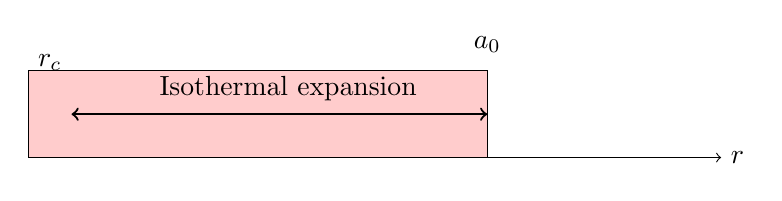
\begin{tikzpicture}[scale=1.1]
                    \draw[->] (0,0) -- (8,0) node[right] {$r$};

                    \draw[fill=blue!30] (0,0.2) rectangle (0.5,0.8);
                    \node at (0.25,1.1) {$r_c$};

                    \draw[fill=red!20] (0,0) rectangle (5.3,1.0);
                    \node at (5.3,1.3) {$a_0$};

                    \draw[<->, thick] (0.5,0.5) -- (5.3,0.5);
                    \node at (3,0.8) {Isothermal expansion};
                \end{tikzpicture}
                \caption{Hydrogen ground-state radius as an isothermal swelling from $\rc$ to $a_0$.}
            \end{figure}

%--------------------------------------------------------------
        \subsection*{F.3 Unruh Echo: Two-Stage Thermodynamic Response}

            \begin{figure}[h!]
                \centering
                \begin{tikzpicture}[scale=1.2]
                    \draw[->] (0,0) -- (7,0) node[right] {$t$};
                    \draw[->] (0,0) -- (0,3) node[above] {Signal};

                    % primary burst
                    \draw[thick] (0.1,0) -- (0.1,2.5);
                    \node at (0.1,2.8) {Primary (0.1 ns)};

                    % echo
                    \draw[thick] (3,0) -- (3,2);
                    \node at (3,2.4) {Echo (30 ns)};
                \end{tikzpicture}
                \caption{SST interpretation of Unruh Echo: fast swirl-sector pulse followed by
                slower EM transduction.}
            \end{figure}

%==============================================================
%% {References}
%==============================================================

        \begin{thebibliography}{99}

            \bibitem{AbeOkuyama}
            S.~Abe and S.~Okuyama,
            ``Similarity between quantum mechanics and thermodynamics:
            Entropy, temperature, and Carnot cycle,''
            Phys.\ Rev.\ E \textbf{83}, 021121 (2011).
            doi:10.1103/PhysRevE.83.021121.

            \bibitem{Kelvin}
            W.~Thomson (Lord Kelvin),
            ``On Vortex Atoms,''
            Proc.\ R.\ Soc.\ Edinburgh (1867).

            \bibitem{Helmholtz}
            H.~Helmholtz,
            ``Über Integrale der hydrodynamischen Gleichungen,''
            J.\ Reine Angew.\ Math.\ \textbf{55}, 25--55 (1858).

            \bibitem{Batchelor}
            G.~K.~Batchelor,
            \emph{An Introduction to Fluid Dynamics},
            Cambridge University Press (1967).

            \bibitem{Saffman}
            P.~G.~Saffman,
            \emph{Vortex Dynamics},
            Cambridge University Press (1992).

            \bibitem{Sornette1998}
            D.~Sornette,
            ``Discrete scale invariance and complex dimensions,''
            Phys.\ Rep.\ \textbf{297}, 239--270 (1998).
            doi:10.1016/S0370-1573(97)00076-8.

            \bibitem{Buchert2000}
            T.~Buchert,
            ``On average properties of inhomogeneous fluids in general relativity: Dust cosmologies,''
            Gen.\ Relativ.\ Gravit.\ \textbf{32}, 105--125 (2000).
            doi:10.1023/A:1001800617177.

            \bibitem{Unruh1976}
            W.~G.~Unruh,
            ``Notes on black-hole evaporation,''
            Phys.\ Rev.\ D \textbf{14}, 870--892 (1976).
            doi:10.1103/PhysRevD.14.870.

            \bibitem{SSTCanon}
            O.~Iskandarani,
            \emph{Swirl--String Theory: Canon v0.5.12},
            Zenodo (2025).

            \bibitem{HydroHydrogen}
            O.~Iskandarani,
            ``Hydrodynamic Origin of the Hydrogen Ground State,''
            Zenodo (2025).

            \bibitem{DualVacuum}
            O.~Iskandarani,
            ``Hydrodynamic Dual-Vacuum Unification: Swirl Radiation and Photon Torsion,''
            Zenodo (2025).

            \bibitem{UnruhEcho}
            O.~Iskandarani,
            ``Two-Vacuum Interpretation of the Unruh Echo,''
            Zenodo (2025).

        \end{thebibliography}

\end{document}